\begin{figure}[!ht]
    \centering
    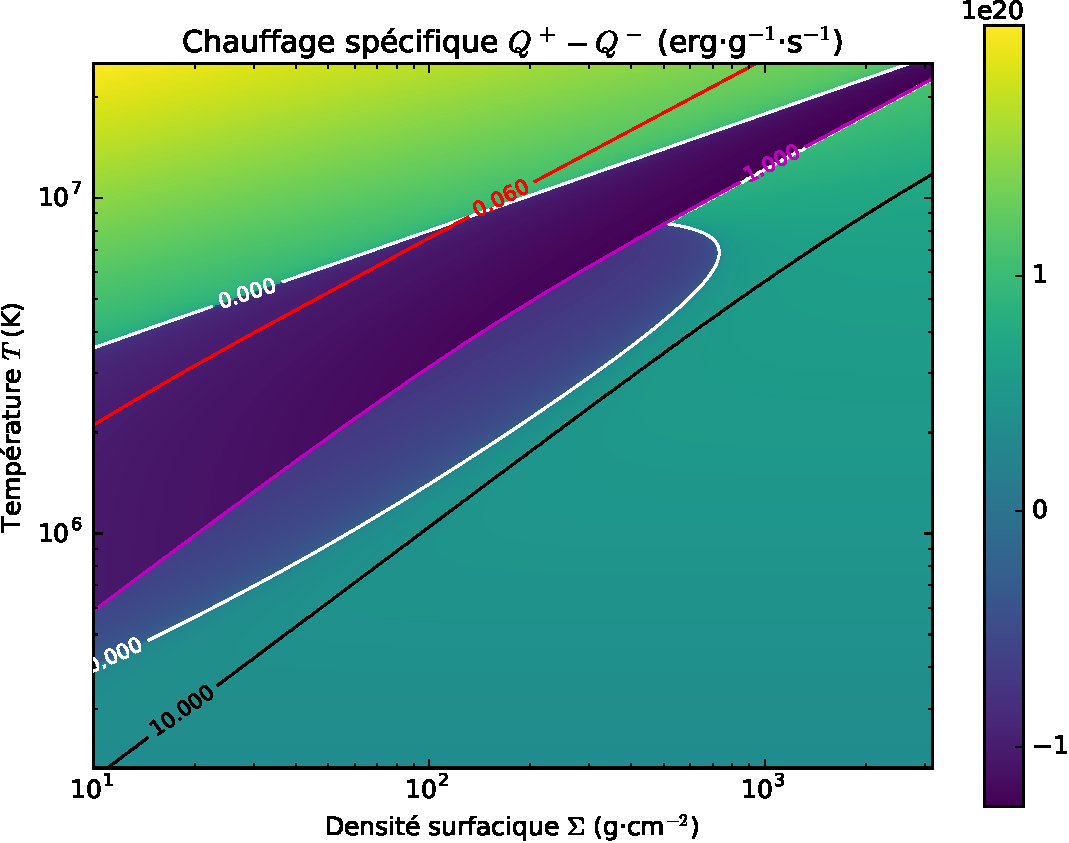
\includegraphics[width=\textwidth]{Qmap.pdf}
    \caption{Carte de la différence des termes de chauffages et de refroidissement en fonction de $T$ et $\Sigma$}
    \label{fig:qmap}
\end{figure}

Sur la \cref{fig:qmap} on aperçoit bien les différentes zones du problèmes et
le comportement du système se prédit bien. On observe d’ailleurs que la courbe
en S est fortement modifiée par la prise en compte effective de l’opacité : la
partie basse se voit bien, la partie haute (droite blanche supérieure)
également, mais la jonction entre les deux ne se fait pas.

En commençant dans la partie stable en bas à gauche, tout point est amené à se
retrouver sur la partie basse de la courbe en S, puisqu’il est chauffé si
en-dessous et refroidi si au-dessus. Ensuite, avec l’accrétion de matière, le
système va remonter le long de cette courbe jusqu’à arriver au premier point
critique.

À partir de cet instant, plus rien ne l’empêche de monter en température, ce
qu’il va donc faire. Dans cette zone, la convection n’est plus négligeable, car
les points du système ne sont plus tous concentrés dans la même zone
d’évolution. On va donc voir une instabilité se propager sous la forme d’un pic
de densité de matière et d’un front de température : la matière en trop au
centre va partir vers l’extérieur, poussant les points restés en bas à droite
du point critique ; ils iront donc rejoindre les autres sur la branche haute.

Cette évolution s’arrête en effet pour tout point dès lors qu’il atteint la
frontière $\tau_{eff} = 1$. Au-dessus de cette barrière le terme de
refroidissement reprend le dessus fortement, et les points se figent.

Puis, une fois l’instabilité dissipée, le système va se refroidir
progressivement en redescendant le long de la droite $\tau_{eff} = 1$, jusqu’à
retomber à « l’intérieur » de la courbe en S. À ce moment-là, plus rien
n’empêche les points de redescendre en température, et ils vont donc retomber
sur la partie basse.
